%%%%%%%%%%%%%%%%%%%%%%%%%%%%%%%%%%%%%%%%%
% Short Sectioned Assignment
% LaTeX Template
% Version 1.0 (5/5/12)
%
% This template has been downloaded from:
% http://www.LaTeXTemplates.com
%
% Original author:
% Frits Wenneker (http://www.howtotex.com)
% Edited by Alice Wu
%
% License:
% CC BY-NC-SA 3.0 (http://creativecommons.org/licenses/by-nc-sa/3.0/)
%
%%%%%%%%%%%%%%%%%%%%%%%%%%%%%%%%%%%%%%%%%

%----------------------------------------------------------------------------------------
%	PACKAGES AND OTHER DOCUMENT CONFIGURATIONS
%----------------------------------------------------------------------------------------

\documentclass[paper=letter, fontsize=11pt]{scrartcl} % letter and 11pt font size
\usepackage[margin=1in]{geometry}
\usepackage[T1]{fontenc} % Use 8-bit encoding that has 256 glyphs
\usepackage{fourier} % Use the Adobe Utopia font for the document - comment this line to return to the LaTeX default
\usepackage[english]{babel} % English language/hyphenation
\usepackage{amsmath,amsfonts,amsthm} % Math packages
\usepackage{comment}
\usepackage{graphicx}
\usepackage{caption}
\usepackage{subcaption}

\usepackage{lipsum} % Used for inserting dummy 'Lorem ipsum' text into the template

\usepackage{sectsty} % Allows customizing section commands
\usepackage{fancyhdr} % Custom headers and footers
\pagestyle{fancyplain} % Makes all pages in the document conform to the custom headers and footers
\fancyhead{} % No page header - if you want one, create it in the same way as the footers below
\fancyfoot[L]{} % Empty left footer
\fancyfoot[C]{} % Empty center footer
\fancyfoot[R]{\thepage} % Page numbering for right footer
\renewcommand{\headrulewidth}{0pt} % Remove header underlines
\renewcommand{\footrulewidth}{0pt} % Remove footer underlines
%\setlength{\headheight}{0pt} % Customize the height of the header

\numberwithin{equation}{section} % Number equations within sections (i.e. 1.1, 1.2, 2.1, 2.2 instead of 1, 2, 3, 4)
%\numberwithin{figure}{section} % Number figures within sections (i.e. 1.1, 1.2, 2.1, 2.2 instead of 1, 2, 3, 4)
%\numberwithin{table}{section} % Number tables within sections (i.e. 1.1, 1.2, 2.1, 2.2 instead of 1, 2, 3, 4)

\setlength\parindent{24pt} % Removes all indentation from paragraphs - comment this line for an assignment with lots of text

%use itlesec package and zero out all the spaces and set it manually
%titlespacing are command, left margin, above-skip and below-kip respectively
\usepackage[compact]{titlesec}
\titlespacing{\section}{0pt}{*2}{*1}
\titlespacing{\subsection}{0pt}{*2}{*1}
\titlespacing{\subsubsection}{0pt}{*2}{*1}

%----------------------------------------------------------------------------------------
%	TITLE SECTION
%----------------------------------------------------------------------------------------

\newcommand{\horrule}[1]{\rule{\linewidth}{#1}} % Create horizontal rule command with 1 argument of height

\title{	
\normalfont \normalsize 
\textsc{Stanford University, CS229 - Machine Learning} \\ [25pt] % Your university, school and/or department name(s)
\horrule{0.5pt} \\[0.4cm] % Thin top horizontal rule
\huge Final Project Milestone - Kicked Car Prediction \\ % The assignment title
\horrule{2pt} \\[0.3cm] % Thick bottom horizontal rule
}

\author{Albert Ho, Robert Romano, X. Alice Wu} % Your name

\date{\normalsize\today} % Today's date or a custom date

\begin{document}
\noindent
\maketitle % Print the title

%----------------------------------------------------------------------------------------
%	PROBLEM 1
%----------------------------------------------------------------------------------------
\section{Introduction}
	When you go to an auto dealership with the intent to buy a used car, you want a good selection to choose from and you want to be able to trust the condition of the car that you buy. Auto dealerships purchase many of their used cars through auto auctions with the same goals that you have: they want to buy as many cars as they can in the best condition possible. The problem that these dealerships often face is the risk of buying used cars that have serious issues, preventing them from being sold to customers. These bad purchases are called "kicks", and they can be hard to spot for a variety of reasons. Many kicked cars are purchased due to tampered odometers or mechanical issues that could not be predicted ahead of time. For these reasons, car dealerships can benefit greatly from the predictive powers of machine learning. If there is a way to determine if a car would be kicked ahead of time, car dealerships can not only save themselves money, but also provide their customers with the best inventory selection possible.

	The following paper is split up into 3 main sections describing our approach to solve this problem: Early Interpretation, Data Parsing, and Machine Learning Algorithms. First we identified possible trends by simply graphing data. Next, we came up with strategies for dealing with missing data and data presented in a text format. Finally, we applied various machine learning algorithms to the parsed data set in an attempt to predict which cars would have the highest risk of being kicked.

\section{Early Interpretation}
	We obtained our data set from the Kaggle.com challenge "Don't Get Kicked" hosted by Carvana. Our first step was to graph the data we had to gain some initial insight into which features would be the most important. The features we were provided along with their descriptions are shown in Table 1. 

\begin{comment}
\begin{table}[!ht]
	\begin{center}
	 \begin{tabular}{ | p{3cm} | p{4cm} | p{3cm} | p{4cm} |}
	 \hline
		{\bf Feature}	& {\bf Short Description} & {\bf Feature	Short} & {\bf Description} \\ \hline
		RefID	& Unique vehicle identifier &	VehOdo & Vehicle Odometer reading \\ \hline
		IsBadBuy & Was the car kicked? & Nationality & Manufacturer's country\\ \hline
		PurchDate & Auction Purchase date & Size & (Compact, SUV, etc.) \\ \hline
		Auction & Auction provider & PrimeUnit & Car has higher demand? \\ \hline
		VehYear & Vehicle year & AcquisitionType & (Auction buy, Trade in, etc.) \\ \hline
		VehicleAge & Years elapsed & VehYear & AucGuart	Guarantee provided by Auction \\ \hline
		Make & Vehicle Manufacturer & ByrNo & Unique identifier for buyer \\ \hline
		Model & Vehicle Model & VnZip & Zipcode of car purchase \\ \hline
		Trim & Vehicle Trim Level & VnSt & State of car purchase \\ \hline
		SubModel & Vehicle Submodel & VehBCost & Acquisition cost to buyer \\ \hline
		Color & Vehicle Color & IsOnlineSale & Was this an online purchase? \\ \hline
		Transmission & Vehicle transmission type & WarrantyCost & Warranty price \\ \hline
		WheelType & Indicates type of wheel & & \\ \hline
	 \end{tabular}
	\end{center}
	
	\begin{center}
	 \begin{tabular}{ | p{6.42cm} | p{8.42cm} |}
	 \hline
		{\bf Feature}	& {\bf Short Description}  \\ \hline
		TopThreeAmericanName & Is manufacturer one of top three? \\ \hline
		MMRAcquisitionAuctionAveragePrice* & Average condition value at auction time \\ \hline
		MMRAcquisitionAuctionCleanPrice* & Great condition value at auction time \\ \hline
		MMRAcquisitionRetailAveragePrice* & Average condition retail value at auction time \\ \hline
		MMRAcquisitionRetailCleanPrice* & Great condition retail value at auction time \\ \hline
		MMRCurrentAuctionAveragePrice* & Average condition value currently \\ \hline
		MMRCurrentAuctionCleanPrice* & Great condition value currently \\ \hline
		MMRCurrentRetailAveragePrice* & Average condition retail value currently \\ \hline
		MMRCurrentRetailCleanPrice* & Great condition retail value currently \\ \hline
	 \end{tabular}
	\end{center}
  \caption{Feature labels and descriptions.}
	\begin{center}
	*MMR refers to Manheim Market Report and is the source of these values
	\end{center}
\end{table}
\end{comment}

\section{Data Parsing}
	Many of the features we were looking at came in a text format, so we had to decide how to properly bin them. Furthermore, some data entries were missing, so we had to make some choices for how to replace them.

\subsection{Word Bins}
	For data such as the name of the vehicle's model, manufacturer, and color, we had to assign unique identifiers to specific strings in the feature space. This was straightforward for a feature like transmission since we could assign 0 for Auto and 1 for manual. The process became more involved with features such as the car submodel. We decided that even though there were many different submodels, categorizing them with unique identifiers rather than grouping them was the more conservative option.

\subsection{Missing Features}
	For many of the samples, particular features were missing. We had the option of throwing out the sample completely, but we believed that it would be a waste. We decided to implement the following rules: if the feature was represented with a continuous value, we would replace the missing value with the average of the feature over the other samples and if the feature was represented with a discrete value, we would create a new value specifically to identify missing data.

\section{Data Visualization}

\begin{comment}
\begin{figure}[!ht]
  \centering
	\includegraphics[width=0.8\columnwidth] %width=0.5\textwidth
		{}
	\caption{blehblehbleh}
\end{figure}
\end{comment}

\begin{figure}[!ht]
        \centering
        \begin{subfigure}[b]{0.5\textwidth}
                \centering
                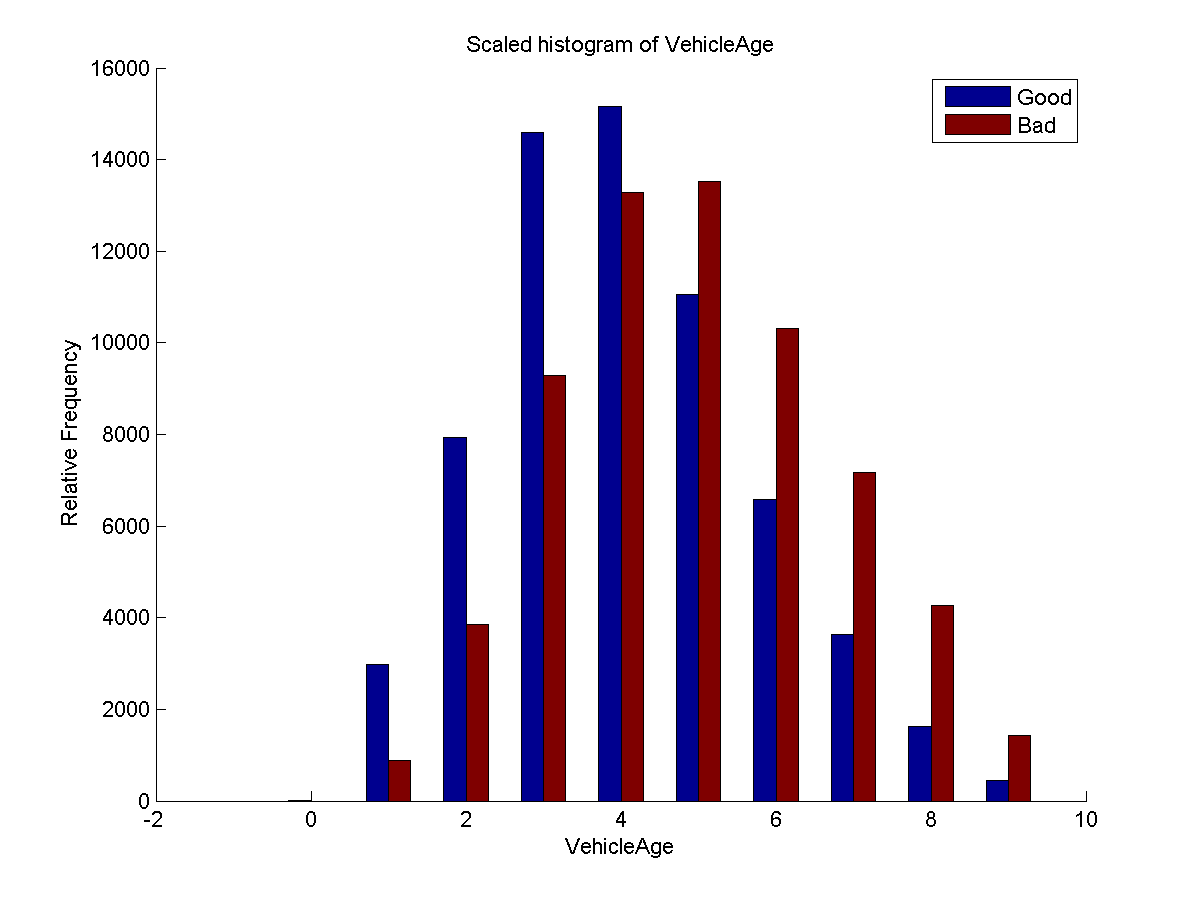
\includegraphics[width=\textwidth]{figures/HistogramScaled_VehicleAge}
                \caption{Ratio of Scaled VehicleAge}
                \label{fig:Scaled_VehicleAge}
        \end{subfigure}%
        ~ %add desired spacing between images, e. g. ~, \quad, \qquad etc. 
          %(or a blank line to force the subfigure onto a new line)
        \begin{subfigure}[b]{0.5\textwidth}
                \centering
                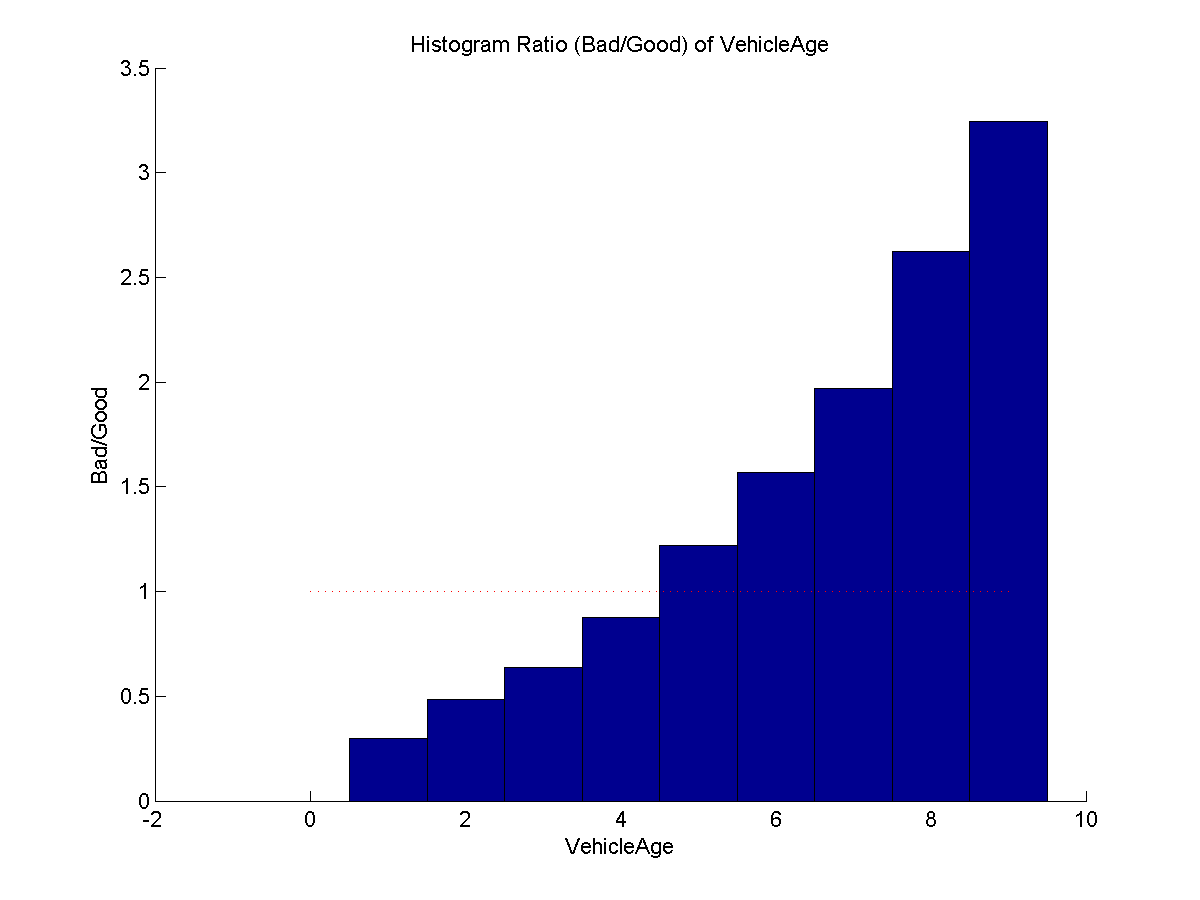
\includegraphics[width=\textwidth]{figures/HistogramRatio_VehicleAge}
                \caption{Ratio of VehicleAge}
                \label{fig:VehicleAge}
        \end{subfigure}
        ~ %add desired spacing between images, e. g. ~, \quad, \qquad etc. 
          %(or a blank line to force the subfigure onto a new line)
        \begin{subfigure}[b]{0.5\textwidth}
                \centering
					 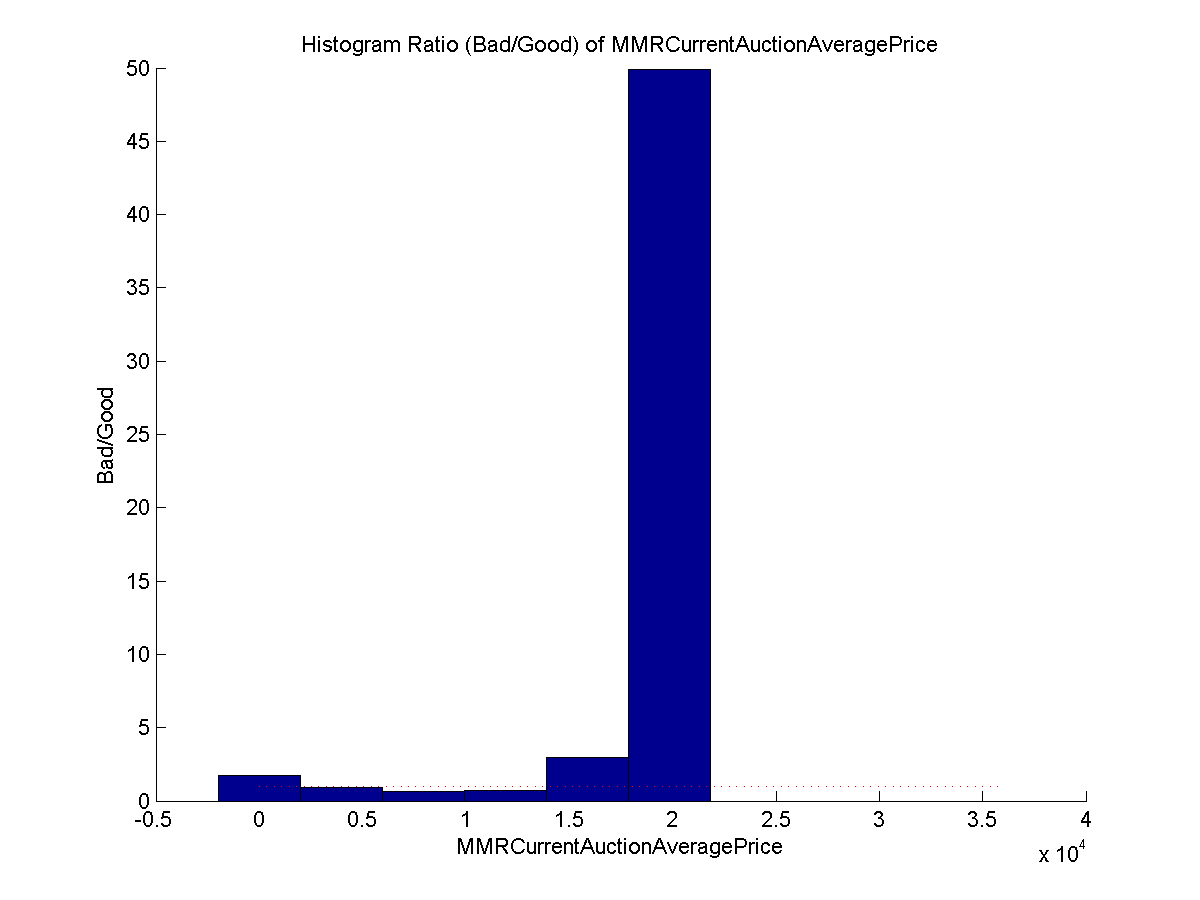
\includegraphics[width=\textwidth]{figures/HistogramRatio_MMRCurrentAuctionAveragePrice.png}
                \caption{Ratio of MMRCurrentAuctionAvgPrice}
                \label{fig:MMRCurrentAuctionAveragePrice}
        \end{subfigure}
        \caption{blehbleblehblehbleh}\label{fig:Histograms}
\end{figure}

\section{Machine Learning Algorithms}
	With the data parsed and some initial insights to guide us, we started to apply some machine learning algorithms that would identify where we needed improvement and what strategy would be most effective.

\subsection{Support Vector Machine}
	First, we tested our data with an SVM. We used the liblinear package v. 1.92. Our initial runs thus far have only been on raw numerical data (not on all post-processed data), so there is lots of room for improvement. We submitted our solution to Kaggle and placed 526 out of 571 teams on our first run.

\subsection{Logistic Regression}
	Since the output of our data is binary, we decided to fit two logistic regression models as a fist pass. Adopting code from the course website and assignment 1, we implemented logistic gradient ascent and Newton's method. Both of the algorithms are run on the numerical training data only. When possible, a 70/30 cross validation was performed. The generalization error is defined as:
\begin{align} 
\begin{split}
\varepsilon(h) &= \frac{\sum|y_{true} - y_{predicted}|}{n} \\
\end{split}					
\end{align}

\subsubsection{Logistic Gradient Ascent}
	Using logistic gradient ascent with a learning rate of alpha = 0.0001 and 500 iterations. We were not able to generate any log-likelihood data past the first iteration. The first 
One possible hypothesis we have about this method is that the data may not be convex

\subsubsection{Newton's Method}
	We first used Newton's method in a 70/30 cross validation scheme. We found that the algorithm converged after 7 iterations, with a relative difference of -1.6007e-010. Although at this point the algorithm was only run on the the numerical data from the total data set, it yielded a generalization error of 0.1178, which is highly promising. However, when the data was visualized 

\end{document}
